\documentclass[10pt,xcolor=pst,aspectratio=169]{beamer}

\usepackage{etex}

%\usetheme{Boadilla}
%\usecolortheme{wolverine}
\usecolortheme{dolphin}
%\setbeamercovered{transparent}
%\setbeamercolor{block body}{bg=yellow}

\addtobeamertemplate{navigation symbols}{}{%
\usebeamerfont{footline}%
\usebeamercolor[fg]{footline}%
\hspace{1em}%
\insertframenumber/\inserttotalframenumber
}

\usepackage[utf8]{inputenc}
\usepackage[english,russian]{babel}
\usepackage[OT1]{fontenc}
\usepackage{amsmath}
\usepackage{amsfonts}
\usepackage{amssymb}
\usepackage{graphicx}
\usepackage{wrapfig}
\usepackage[3D]{movie15}
\usepackage{ragged2e}
\usepackage{listings}
\usepackage{color}
\usepackage{pst-all}

\usepackage{tikz}
\usetikzlibrary{
	mindmap,
	arrows, % стрелки
	shapes.misc, % фигуры
	chains, % цепочки
	positioning, % позиционирование элементов
	scopes, % создание дополнительных веток
	shadows % тени
	}

\graphicspath{{pic/}}

\author{\textbf{Губкин А.С.}}

\title[Численные методы в физике]{Численные методы в физике}

\logo{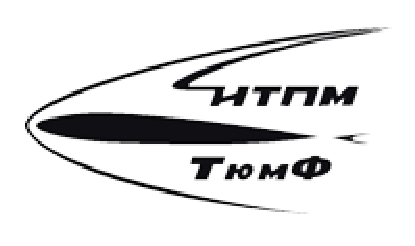
\includegraphics[width=0.1\linewidth]{LOGO_2.EPS}}

\institute[ТюмФ ИТПМ СО РАН]{Тюменский филиал Института теоретической и прикладной механики\\ им. С. А. Христиановича СО РАН, г. Тюмень}

%\date{6 октября 2015 г.}

\begin{document}

\lstset{ %
	language=[ANSI]C++,                 % выбор языка для подсветки (здесь это С++)
	keywordstyle=\color{blue},
	commentstyle=\color{gray},
	basicstyle=\scriptsize,
%basicstyle=\small\sffamily, % размер и начертание шрифта для подсветки кода
	numbers=left,               % где поставить нумерацию строк (слева\справа)
	numberstyle=\tiny,           % размер шрифта для номеров строк
%stepnumber=1,                   % размер шага между двумя номерами строк
	numbersep=4pt,                % как далеко отстоят номера строк от подсвечиваемого кода
%backgroundcolor=\color{white}, % цвет фона подсветки - используем \usepackage{color}
	showspaces=false,            % показывать или нет пробелы специальными отступами
	showstringspaces=false,      % показывать или нет пробелы в строках
	showtabs=false,             % показывать или нет табуляцию в строках
	frame=single,              % рисовать рамку вокруг кода
%tabsize=2,                 % размер табуляции по умолчанию равен 2 пробелам
	captionpos=t,              % позиция заголовка вверху [t] или внизу [b] 
	breaklines=true,           % автоматически переносить строки (да\нет)
	breakatwhitespace=true, % переносить строки только если есть пробел
	escapeinside={\%*}{*)}   % если нужно добавить комментарии в коде
}

%SLIDE #
\begin{frame}

	\transdissolve[duration=0.1]
	\titlepage

\end{frame}

%SLIDE #
\begin{frame}{Литература}

	\transdissolve[duration=0.1]

    \begin{itemize}
        \item Андерсон Д., Таннехилл Дж., Плетчер Р. Вычислительная гидродинамика и теплообмен. Том 1,2 (1990).

        \item Зализняк В.Е. Численные методы. Основы научных вычислений. - М.: Издательство Юрайт, 2012. - 356 с.

        \item Формалев В.Ф., Ревезников Д.Л. Численные методы. - М.: ФИЗМАТЛИТ, - 2004. - 400 с.

        \item Рождественский Б.Л., Яненко Н.Н. Системы квазилинейных уравнений и их приложения к газовой динамике (2-е изд.). - М.: Наука, 1978. - 688 с.
        
        \item Жуков М.Ю. Квазилинейные гиперболические уравнения: Учебно-методическое пособие. - Ростов-на-Дону, 2008. - 52 с.

        \item Куликовский А.Г., Погорелов Н.В., Семенов А.Ю. Математические вопросы численного решения гиперболических систем уравнений. - М.: ФИЗМАТЛИТ, 2012. - 656 с.

        \item Лейбович С., Сибасс А. (ред.) Нелинейные волны. - М.: Мир, 1977.
    \end{itemize}

    и др.

\end{frame}

%SLIDE #
\begin{frame}{Введение}

	\transdissolve[duration=0.1]
	\justifying
	\large

	Многие физические проблемы сводятся к решению \textbf{уравнений в частных производных}, поэтому необходимо знать физические особенности решений этих уравнений. Для решения конкретных задач необходимо уметь определять тип дифференциального уравнения в частных производных и знать его основные математические особенности.

\end{frame}

%SLIDE #
\begin{frame}{Уравнение в частных производных}

	\transdissolve[duration=0.1]
	\justifying
	\large

	Уравнением в частных производных относительно функции $u \left( \vec{x} \right)$ называется уравнение вида:

	\[
		f \left( \vec{x}, u, \frac{\partial u}{\partial \vec{x}}, \frac{\partial^{2} u}{\partial \vec{x} \partial \vec{x}}, \ldots \right) = 0.
	\]

\end{frame}

%SLIDE #
\begin{frame}{Физическая классификация уравнений}

	\transdissolve[duration=0.1]
	\justifying
	\large

%	\begin{center}
%		\begin{tikzpicture}[edge from parent fork down]
%			\tikzstyle{every node}=[fill=yellow!150, rounded corners]
%			\tikzstyle{edge from parent}=[blue, -*, thick,draw]
%			\tikzstyle{level 1}=[level distance=2cm, sibling distance=4cm]
%			
%			\node {Задачи для УЧП}
%				child {node {Маршевые}}
%				child {node {Стационарные}};
%		\end{tikzpicture}
%	\end{center}
	
	\begin{center}
		\tikzstyle{root concept}+=[concept color=blue!80,minimum size=3cm]
		\tikz[mindmap]
			\node [concept] {Задачи для УЧП}
				child[concept color=yellow, grow=135, minimum size=2cm]
				{
					node[concept](root1) at (1,0) {Маршевые} node[annotation,left] at (0,0)
					{
						\begin{itemize}
							\item нестационарные течения невязкой/вязкой жидкости;
							\item стационарные сверхзвуковые течения невязкого/вязкого газа;
							\item пограничный слой;
							\item нестационарное распространение тепла, и т.д.
						\end{itemize}
					}
				}
				child[concept color=green, grow=45, minimum size=2cm] 
				{
					node[concept](root2) at (-1,0) {Стацио\-нарные} node[annotation,right] at (0,0)
					{
						\begin{itemize}
							\item стационарные течения невязкой/вязкой жидкости;
							\item стационарные сверхзвуковые течения невязкого/вязкого газа;
							\item стационарные задачи теплопроводности, и т.д.
						\end{itemize}
					}
				};
	\end{center}

\end{frame}

%SLIDE #
\begin{frame}{Маршевые задачи}

	\transdissolve[duration=0.1]
	\justifying
	\large

	\textbf{Маршевой} или \textbf{эволюционной} (или задачей распространения) называется задача, в которой требуется найти решение уравнения в частных производных в \textbf{незамкнутой области} при заданных граничных и начальных условиях.\\

	Решение таких задач должно быть найдено последовательным движением в маршевом направлении. Такие задачи описываются уравнениями в частных производных \textbf{гиперболического} или \textbf{параболического} типа.

\end{frame}

%SLIDE #
\begin{frame}{Стационарные}

	\transdissolve[duration=0.1]
	\justifying
	\large

	Задача называется \textbf{стационарной}, если решение уравнения в частных производных внутри некоторой области определяется лишь условиями на границе этой области\\

	Физически стационарная задача описывает установившийся процесс, а математически сводится к решению задачи с граничными условиями (краевой задачи) для уравнения в частных производных.\\

	Иногда стационарные задачи называют \textbf{детерминированными}, так как решение в любой внутренней точке области определяется условиями, заданными на ее границе.

\end{frame}

%SLIDE #
\begin{frame}{Уравнения характерные для маршевых задач}

	\transdissolve[duration=0.1]
	\justifying
	\large

    Волновое уравнение:

	\[
		a(\vec{x}) \frac{\partial^{2} u}{\partial t^{2}} = \vec{\nabla} \cdot \left( b(\vec{x}) \vec{\nabla} u \right) - c(\vec{x}) u + f(\vec{x}, t).
	\]

	Уравнение теплопроводности (диффузии):

	\[
		a(\vec{x}) \frac{\partial u}{\partial t} = \vec{\nabla} \cdot \left( b(\vec{x}) \vec{\nabla} u \right) - c(\vec{x}) u + f(\vec{x}, t).
	\]

\end{frame}

%SLIDE #
\begin{frame}{Уравнения характерные для маршевых задач}

	\transdissolve[duration=0.1]
	\justifying
	\large

	Уравнения Максвелла:

	\[
		\begin{split}
			&\vec{\nabla} \cdot \vec{D} = \rho (\vec{x}), \:
			\vec{\nabla} \cdot \vec{B} = 0 \\ 
			&\vec{\nabla} \times \vec{E} = - \frac{\partial \vec{B}}{\partial t}, \:
			\vec{\nabla} \times \vec{H} = \vec{j} + \frac{\partial \vec{D}}{\partial t}.
		\end{split}
	\]

\end{frame}

%SLIDE #
\begin{frame}{Уравнения характерные для маршевых задач}

	\transdissolve[duration=0.1]
	\justifying
	\large

	Уравнения газо-гидродинамики (уравнения Эйлера):

	\[
		\begin{split}
			&\frac{\partial \rho}{\partial t}
				+ \vec{\nabla} \cdot \rho \vec{u}
				= 0, \\
			&\frac{\partial \rho \vec{u}}{\partial t}
				+ \vec{\nabla} \cdot \left( \rho \vec{u} \otimes \vec{u} + p \textbf{I} \right)
				=
				\vec{F}, \\
			&\frac{\partial \rho E}{\partial t}
				+ \vec{\nabla} \cdot \left( \vec{u} \left( \rho E + p \right) \right)
				=
				\vec{F} \cdot \vec{u}.
			\end{split}
	\]

\end{frame}

%SLIDE #
\begin{frame}{Уравнения характерные для маршевых задач}

	\transdissolve[duration=0.1]
	\justifying
	\large

    Уравнения Навье-Стокса:
	\[
		\begin{split}
			&\frac{\partial \rho}{\partial t}
				+ \vec{\nabla} \cdot \rho \vec{u}
				= 0, \\
			&\frac{\partial \rho \vec{u}}{\partial t}
				+ \vec{\nabla} \cdot \rho \vec{u} \otimes \vec{u}
				=
				- \vec{\nabla} p
				+ \vec{\nabla} \cdot \tau
				+ \vec{F}, \\
			&\frac{\partial \rho E}{\partial t}
				+ \vec{\nabla} \cdot \rho E \vec{u}
				=
				\vec{\nabla} \cdot \left( \sigma \cdot \vec{u} - \vec{q} \right)
				+ \vec{F} \cdot \vec{u}.
			\end{split}
	\]

\end{frame}

%SLIDE #
\begin{frame}{Уравнения характерные для стационарных задач}

	\transdissolve[duration=0.1]
	\justifying
	\large

    Волновое уравнение и уравнение диффузии:
   
	\[
		\vec{\nabla} \cdot \left( b(\vec{x}) \vec{\nabla} u \right) - c(\vec{x}) u + f(\vec{x}, t) = 0.
	\]

    Уравнение Гельмгольца:

	\[
		\triangle u_{0} + \frac{\omega^{2}}{c^2} u_{0} = - \frac{f_{0}(\vec{x})}{c^{2}}.
	\]

    Уравнения электростатики и магнитостатики:

	\[
		\begin{split}
			&\vec{\nabla} \cdot \vec{D} = \rho (\vec{x}), \:
			\vec{\nabla} \times \vec{E} = 0, \\
			&\vec{\nabla} \cdot \vec{B} = 0, \:
			\vec{\nabla} \times \vec{H} = \vec{j}.
		\end{split}
	\]

\end{frame}

%SLIDE #
\begin{frame}{Постановка основных задач для уравнений математической физики}

	\transdissolve[duration=0.1]
	\justifying
	\large

	Различают три основных типа краевых задач для дифференциальных уравнений в частных производных:

	\begin{itemize}
		\item \textbf{задача Коши} для нестационарных уравнений: задаются начальные условия, граничные условия отсутствуют;

		\item \textbf{краевая задача} для стационарных уравнений: задаются граничные условия, начальные условия отсутствуют;

		\item \textbf{смешаная задача} для нестационарных уравнений: задаются и начальные, и граничные условия.
	\end{itemize}

\end{frame}

%SLIDE #
\begin{frame}{Задача Коши}

	\transdissolve[duration=0.1]
	\justifying
	\large

	\begin{itemize}
		\item Для волнового уравнения второго порядка:
			\[
				u(\vec{x}, 0) = f_{0}(\vec{x}), \: \left. \frac{\partial u(\vec{x}, t)}{\partial t} \right|_{t = 0}= f_{1}(\vec{x}).
			\]

		\item Для уравнений диффузии и Шредингера:
			\[
				u(\vec{x}, 0) = f_{0}(\vec{x}).
			\]

		\item Для системы уравнений первого порядка:
			\[
				\vec{u}(\vec{x}, 0) = \vec{f}_{0}(\vec{x}).
			\]
	\end{itemize}

\end{frame}

%SLIDE #
\begin{frame}{Краевая задача для стационарных уравнений}

	\transdissolve[duration=0.1]
	\justifying
	\large

	Для уравнения 

	\[
		\vec{\nabla} \cdot \left( b(\vec{x}) \vec{\nabla} u \right) - c(\vec{x}) u + f(\vec{x}, t) = 0,
	\]

	граничное условие будет иметь вид:

	\[
		\left. \left( \alpha u + \beta \frac{\partial u}{\partial \vec{n}} \right) \right|_{s} = g_{0}.
	\]

\end{frame}

%SLIDE #
\begin{frame}{Краевая задача для стационарных уравнений}

	\transdissolve[duration=0.1]
	\justifying
	\large

	Часто встречаются следующие типы граничных условий:

	\begin{itemize}
		\item Граничное условие первого рода ($\alpha = 1, \: \beta = 0$):
			\[
				\left. u \right|_{S} = g_{0}.
			\]

		\item Граничное условие второго рода ($\alpha = 0, \: \beta = 1$):
			\[
				\left. \frac{\partial u}{\partial \vec{n}} \right|_{S} = g_{0}.
			\]

		\item Граничное условие третьего рода ($\alpha \geq 0, \: \beta = 1$):
			\[
				\left. \left( \alpha u + \frac{\partial u}{\partial \vec{n}} \right) \right|_{S} = g_{0}.
			\]
	\end{itemize}

\end{frame}

%SLIDE #
\begin{frame}{Математическая классификация уравнений}

	\transdissolve[duration=0.1]
	\justifying
	\large

	Уравнение в частных производных второго порядка, записанное в общем виде, обычно используют для пояснения математической классификации уравнений в частных производных. Рассмотрим уравнение в частных производных

	\[
		a \phi_{xx} + b \phi_{xy} + c \phi_{yy} + d \phi_{x} + e \phi_{y} + f \phi = g(x,y).
	\]

	Здесь $a, \: b, \: c, \: d, \: e, \: f$ -- функции от $x$, $y$, т. е. рассматривается лишь линейное уравнение.

\end{frame}

%SLIDE #
\begin{frame}{Математическая классификация уравнений}

	\transdissolve[duration=0.1]
	\justifying
	\large

	Определим теперь \textbf{канонические} формы записи уравнений в частных производных различных типов.\\

	Известно, что предыдущее уравнение может быть трех различных типов в зависимости от знака определителя:

	\[
		\triangle = b^{2} - 4 a c.
	\]

	\begin{itemize}
		\item гиперболическим: $\triangle > 0$;
		\item параболическим: $\triangle = 0$;
		\item эллиптическим: $\triangle < 0$.
	\end{itemize}

\end{frame}

%SLIDE #
\begin{frame}{Геометрическая аналогия}

	\transdissolve[duration=0.1]
	\justifying
	\large

	\vspace{-60pt}

	\[
    	A x^{2} + B x y + C y^{2} + D x + E y + F = 0.
	\]

    %FIG. #
    \begin{wrapfigure}[10]{r}[-40pt]{8cm}
        \vspace{-20pt}
	    \center{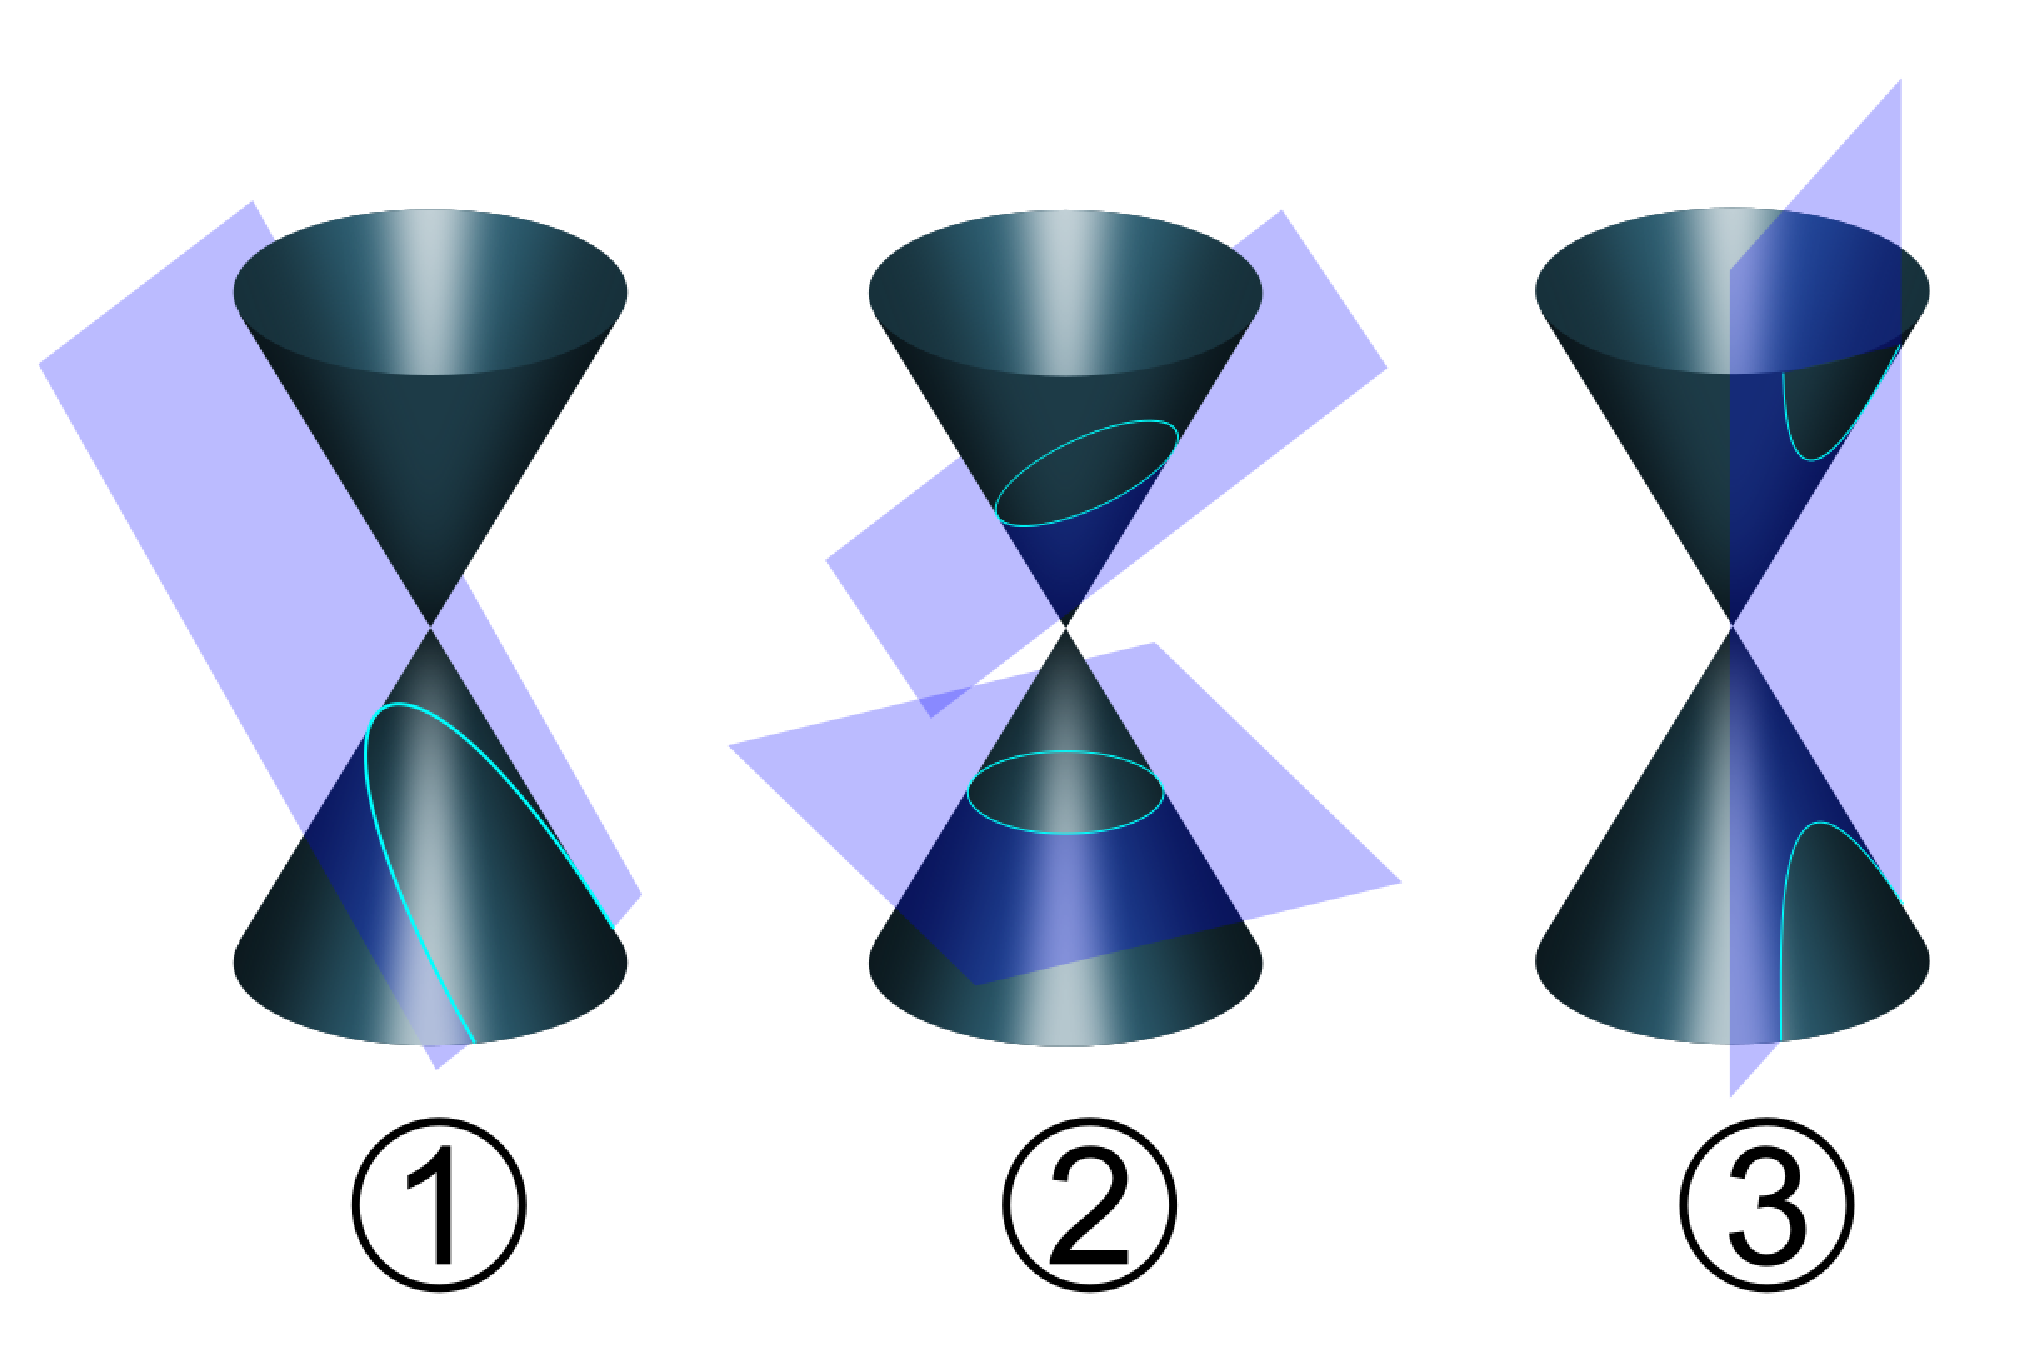
\includegraphics[width=1\linewidth]{conic_sections_with_plane.eps}}
    \end{wrapfigure}

	\[
	    \begin{split}
    	    &B^{2} - 4 A C = 0 \\
    	    &B^{2} - 4 A C < 0 \\
    	    &B^{2} - 4 A C > 0
    	\end{split}
	\]

\end{frame}

%SLIDE #
\begin{frame}{Каноническая форма уравнения}

	\transdissolve[duration=0.1]
	\justifying
	\large

	\begin{itemize}
		\item Каноническая форма уравнения гиперболического типа:
		    \[
			    \phi_{\xi \xi} - \phi_{\eta \eta} = h_{1}(\phi_{\xi}, \phi_{\eta}, \phi, \xi, \eta).
		    \]

		\item Каноническая форма уравнения параболического типа:
		    \[
			    \phi_{\xi \xi} = h_{2}(\phi_{\xi}, \phi_{\eta}, \phi, \xi, \eta).
		    \]

		\item Каноническая форма уравнения эллиптического типа:
		    \[
			    \phi_{\xi \xi} + \phi_{\eta \eta} = h_{3}(\phi_{\xi}, \phi_{\eta}, \phi, \xi, \eta).
		    \]
	\end{itemize}

\end{frame}

%SLIDE #
\begin{frame}{Системы уравнений}

	\transdissolve[duration=0.1]
	\justifying
	\large

	При изучении физических процессов обычно приходится решать \textbf{системы уравнений в частных производных}, так как редко удается описать сложный физический процесс одним уравнением в частных производных. Но даже в тех случаях, когда физический процесс описывается одним уравнением в частных производных высокого порядка, это уравнение можно заменить системой уравнений первого порядка.

\end{frame}

%SLIDE #
\begin{frame}{Пример №1}

	\transdissolve[duration=0.1]
	\justifying
	\large

	В волновом уравнении $\frac{\partial^{2} u}{\partial t^{2}} - c^{2} \frac{\partial^{2} u}{\partial x^{2}} = 0$ сделаем замену:

	\[
		\begin{split}
			&v = \frac{\partial u}{\partial t},\\
			&w = c \frac{\partial u}{\partial x},
		\end{split}
	\]

	тогда уравнение расщипится на систему двух уравнений:

	\[
		\begin{cases}
			&\frac{\partial v}{\partial t} = c \frac{\partial w}{\partial x}, \\
			&\frac{\partial w}{\partial t} = c \frac{\partial v}{\partial x}. \\
		\end{cases}
	\]
	
\end{frame}

%SLIDE #
\begin{frame}{Пример №2}

	\transdissolve[duration=0.1]
	\justifying
	\large

	Запишем уравнение Лапласа $\frac{\partial^{2} u}{\partial x^{2}} + \frac{\partial^{2} u}{\partial y^{2}} = 0$ в виде системы дифференциальных уравнений первого порядка:

	\[
		\begin{cases}
			&\frac{\partial u}{\partial x} = \frac{\partial v}{\partial y},\\
			&\frac{\partial u}{\partial y} = -\frac{\partial v}{\partial x}.
		\end{cases}
	\]

	Это известные уравнения Коши -- Римана, широко используемые в теории конформных отображений.

\end{frame}

%SLIDE #
\begin{frame}{Системы уравнений в частных производных первого порядка}

	\transdissolve[duration=0.1]
	\justifying
	\large

	Так как многие задачи математической физики сводятся к решению \textbf{систем уравнений в частных производных первого порядка}, то для корректной постановки задач необходимо уметь определять \textbf{тип системы уравнений} в частных производных. Рассмотрим систему линейных уравнений в частных производных первого порядка:

	\[
		\frac{\partial \vec{u}}{\partial t} + \textbf{A} \frac{\partial \vec{u}}{\partial x} + \textbf{B} \frac{\partial \vec{u}}{\partial y} + \vec{r} = 0.
	\]

\end{frame}

%SLIDE #
\begin{frame}{Условие гиперболичности системы уравнений в частных производных первого порядка}

	\transdissolve[duration=0.1]
	\justifying
	\large

	Системы уравнений в частных производных первого порядка называется \textbf{гиперболической} по $(x,t)$, если все \textbf{собственные значения} матрицы $\textbf{А}$ \textbf{вещественны и различны}.\\

	То же самое можно сказать о поведении системы уравнений по $(y,t)$ в зависимости от собственных значений матрицы $\textbf{B}$.

\end{frame}

%SLIDE #
\begin{frame}{Пример №3}

	\transdissolve[duration=0.1]
	\justifying
	\large

	В качестве примера рассмотрим систему уравнений из примера №1, записанную в виде:

	\[
		\frac{\partial \vec{u}}{\partial t} + \textbf{A} \frac{\partial \vec{u}}{\partial x} = 0,
	\]

	где

	\[
		\vec{u}
		=
		\begin{bmatrix}
			v \\
			w
		\end{bmatrix}, \:
		\textbf{A}
		=
		\begin{bmatrix}
			0 & - c \\
			-c & 0
		\end{bmatrix}.
	\]

\end{frame}

%SLIDE #
\begin{frame}{Пример №3}

	\transdissolve[duration=0.1]
	\justifying
	\large

	Собственные значения $\lambda$ матрицы $\textbf{A}$ определяются из решения уравнения:

	\[
		\det \left| \textbf{A} - \lambda \textbf{I} \right| = 0.
	\]

	В нашем случае:

	\[
		\begin{Vmatrix}
			- \lambda & - c \\
			-c & - \lambda
		\end{Vmatrix}
		= 0
		\Rightarrow \lambda^2 - c^{2} = 0
		\Rightarrow \lambda_{1,2} = \pm c.
	\]

	\textbf{Система гиперболическая!}

\end{frame}

%SLIDE #
\begin{frame}{Условие эллиптичности системы уравнений в частных производных первого порядка}

	\transdissolve[duration=0.1]
	\justifying
	\large

	Системы уравнений в частных производных первого порядка называется \textbf{эллиптической} по $(x,t)$, если все \textbf{собственные значения} матрицы $\textbf{А}$ \textbf{комплексные}.\\

	То же самое можно сказать о поведении системы уравнений по $(y,t)$ в зависимости от собственных значений матрицы $\textbf{B}$.

\end{frame}

%SLIDE #
\begin{frame}{Пример №4}

	\transdissolve[duration=0.1]
	\justifying
	\large

	В качестве примера рассмотрим систему уравнений Коши -- Римана из примера №2, записанную в виде:

	\[
		\frac{\partial \vec{w}}{\partial x} + \textbf{A} \frac{\partial \vec{w}}{\partial y} = 0,
	\]

	где

	\[
		\vec{u}
		=
		\begin{bmatrix}
			u \\
			v
		\end{bmatrix}, \:
		\textbf{A}
		=
		\begin{bmatrix}
			0 & - 1 \\
			1 & 0
		\end{bmatrix}.
	\]

\end{frame}

%SLIDE #
\begin{frame}{Пример №4}

	\transdissolve[duration=0.1]
	\justifying
	\large

	Собственные значения $\lambda$ матрицы $\textbf{A}$ равны:

	\[
		\begin{Vmatrix}
			- \lambda & - 1 \\
			1 & - \lambda
		\end{Vmatrix}
		= 0
		\Rightarrow \lambda^2 + 1 = 0
		\Rightarrow \lambda_{1,2} = \pm i.
	\]

	\textbf{Система эллиптическая!}

\end{frame}

%SLIDE #
\begin{frame}{Замечание №1}

	\transdissolve[duration=0.1]
	\justifying
	\large

	Система уравнений в частных производных первого порядка может оказаться \textbf{эллиптической} по $(y,t)$ и \textbf{гиперболической} по $(x,t)$ в зависимости от собственных значений матриц $\textbf{B}$ и $\textbf{A}$. Это связано с тем, что тип системы уравнений в частных производных первого порядка по $(x,t)$ и по $(y,t)$ определяется независимо.

\end{frame}

%SLIDE #
\begin{frame}{Замечание №2}

	\transdissolve[duration=0.1]
	\justifying
	\large

	Что делать, когда часть собственных чисел вещественные, а часть комплексные?\\

	Система уравнений c таким характеристическим уравнением смешанная и может обладать свойствами, характерными одновременно для гиперболических, параболических и эллиптических уравнений.\\

	Понять основные свойства решений систем уравнений смешанного типа обычно помогает знание описываемых ими физических процессов.

\end{frame}

\end{document}